\section{Pianificazione}
	\label{pianificazione}
	\subsection{Descrizione}

		Per la realizzazione di \ProjectName{}, il gruppo \GroupName{} 
		ha pianificato il lavoro in cinque diversi periodi basandosi sulle 
		scadenze riportate nella sezione §\ref{subsec:scadenze} a pagina~\pageref{subsec:scadenze}. Queste sono raggruppate
		in due macro-periodi:

		\begin{enumerate}
			\item periodo di formazione:
                \begin{itemize}
                    \item analisi;
                    \item analisi in dettaglio.
                \end{itemize}
			\item periodo contabilizzato:
                \begin{itemize}
                    \item progettazione architetturale;
                    \item progettazione in dettaglio e codifica;
                    \item validazione e collaudo.
                \end{itemize}
		\end{enumerate}
		
		Ognuno di questi periodi è inoltre scomposto in più attività che, in 
		alcuni casi, possono essere eseguite in parallelo. Al 
		termine di ogni periodo vi è una milestone, la quale 
		comporta che tutto il materiale prodotto nelle attività sia 
		pronto per la consegna. 
		Per lasciare un margine nei tempi previsti, nel caso di eventuali 
		ritardi nelle attività, sono stati inseriti dei 
		\glossaryItem{periodi di slack}.

	\subsection{Analisi}
	\label{pianificazioneAnalisi}
        L'inizio di questa attività coincide con la formazione del gruppo e
        l'avvio del progetto, in data 2017-11-10, e si conclude con la
        consegna dei documenti per accedere alla \RR{} in data
        2018-01-16. L'analisi consiste nella scelta di un capitolato proposto,
        incontri con la \glossaryItem{Proponente} per chiarimenti e per la stesura 
        dell'\AnalisiRequisiti{}, e la preparazione dei documenti necessari
        a diventare ufficialmente fornitori. \\
        Questi in particolare sono:

            \begin{itemize}
                \item \textbf{\NormeProgetto{}:}
                    questo documento descrive le regole, gli strumenti e le convenzioni
                    che il gruppo \GroupName{} deve rispettare nello sviluppo del
                    prodotto. Esso ha un importanza critica e
                    va quindi completato prima di cominciare il resto della documentazione;
                \item \textbf{\StudioFattibilita{}:}
                    questo documento contiene un'analisi dei capitolati proposti ed è
                    fondamentale per la scelta del capitolato;
                \item \textbf{\AnalisiRequisiti{}:}
                    questo documento studia in modo più approfondito i requisiti e i casi d'uso
                    del capitolato scelto;
                \item \textbf{\PianoProgetto{}:}
                    questo documento pianifica tutte le attività inerenti al progetto al fine di
                    garantirne un buon esito;
                \item \textbf{\PianoQualifica{}:}
                    questo documento individua i metodi necessari a garantire la qualità del lavoro e comprende i test
                    necessari a garantire la qualità del prodotto;
                \item \textbf{\Glossario{}:}
                    questo documento definisce tutti i termini ritenuti ambigui nella documentazione redatta;
                \item \textbf{Lettera di Presentazione:}
                    questo documento presenta il gruppo \GroupName{} alla Proponente.
            \end{itemize}
	
            \begin{figure}[H]
                \centering
                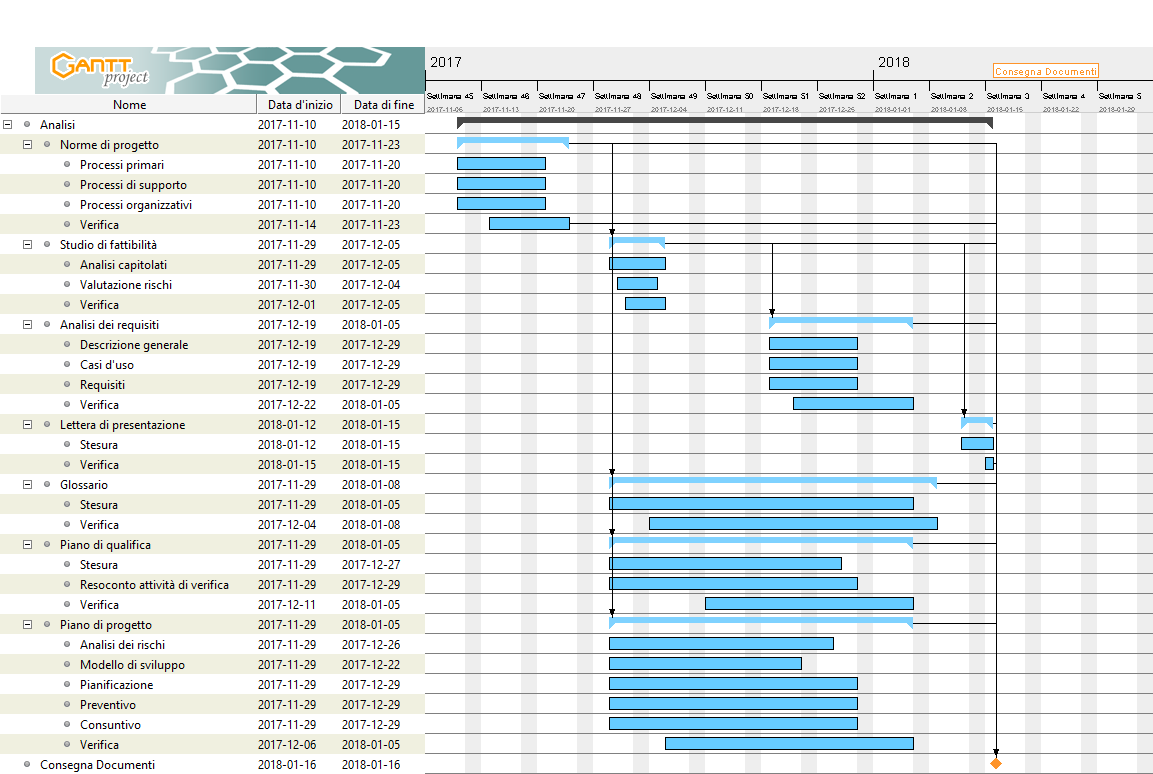
\includegraphics[width=1\linewidth]{./img/Gantt/Analisi.png}
                \caption[Gantt - Analisi]{Diagramma di Gantt: Periodo di Analisi}
            \end{figure}
	
	\newpage 	
	
	\subsection{Analisi in dettaglio}
	\label{pianificazioneAnalisiDettaglio}
		Successivamente alla consegna dei documenti necessari per la candidatura alla
		\RR{}, in data 2018-01-16, viene preparata una presentazione riguardo al prodotto \ProjectName{} e a come il
		gruppo ha lavorato, che verrà utilizzata in data 2018-01-26.
	
            \begin{figure}[H]
                \centering
                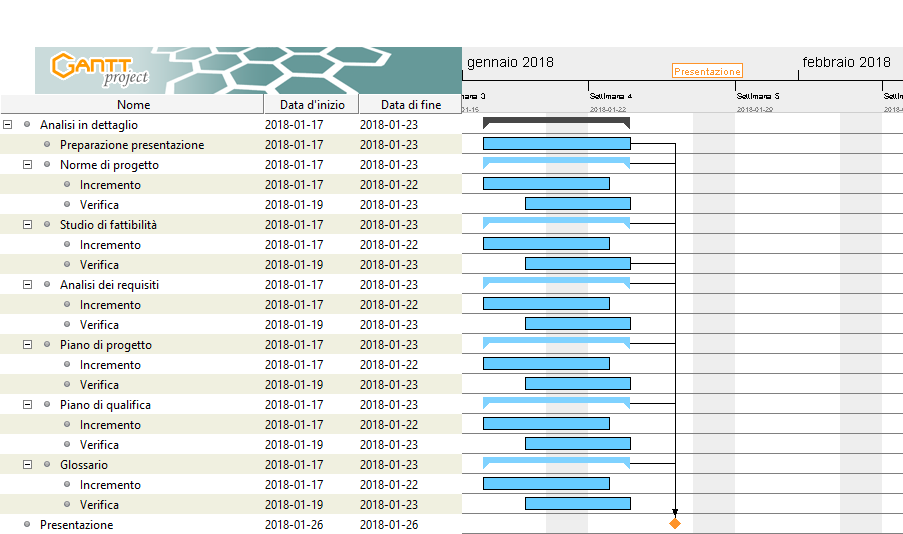
\includegraphics[width=1\linewidth]{./img/Gantt/AnalisiInDettaglio.png}
                \caption[Gantt - Analisi in dettaglio]{Diagramma di Gantt: Periodo di Analisi in Dettaglio}
            \end{figure}
	
	\newpage
	
	\subsection{Progettazione architetturale}
	\label{pianificazioneProgettazione}
		Successivamente al periodo di formazione vi è la progettazione di un'architettura
		adeguata al progetto. Questa comincia il 2018-01-27 e si conclude con la consegna del materiale 
		richiesto per la \RP{} e la discussione della \TecnologyBaseline{}, prevista per 
		il 2018-03-19 (consegna materiale 2018-03-12).\\
		Le principali attività di questo periodo sono:

            \begin{itemize}
                \item \textbf{Incremento e verifica dei documenti precedenti:}
                    miglioramento dei documenti \NormeProgetto{}, \AnalisiRequisiti{},
                    \PianoProgetto{}, \PianoQualifica{}, \Glossario{}. In particolare, per quanto riguarda
                    l'\AnalisiRequisiti{} sono stati negoziati alcuni requisiti opzionali e sono state aggiunte
                    delle sezioni significative. Queste informazioni possono essere trovate dentro al documento \vAnalisiDeiRequisiti{}
                    oppure nel verbale esterno del 2 Marzo 2018;
                \item \textbf{Stesura di nuovi documenti:}
                    viene preparato il semi-elaborato \TecnologyBaseline{} che presenta le
                    tecnologie, i framework e le librerie utilizzate
                    nello sviluppo del prodotto;
                \item \textbf{Creazione del Proof of Concept:} questo prodotto giustifica le scelte tecnologiche
                    fatte nella \TecnologyBaseline{} e mostra il funzionamento dell'architettura scelta;
                \item \textbf{Presentazione e discussione:}
                    al fine di essere ammessi alla \RP{},
                    il gruppo \GroupName{} deve discutere in maniera \glossaryItem{Agile}
                    le proprie scelte architetturali con il professor Riccardo Cardin.
            \end{itemize}
		
		
            \begin{figure}[H]
                \centering
                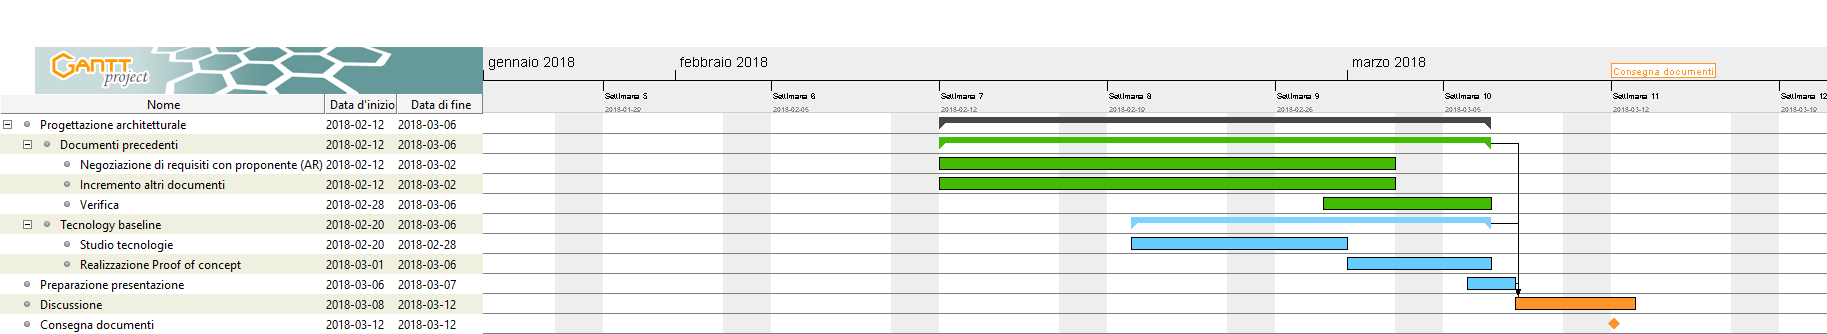
\includegraphics[width=1\linewidth, height=5cm]{./img/Gantt/ProgettazioneArchitetturale.png}

                \caption[Gantt - Progettazione architetturale]{Diagramma di Gantt: Periodo di Progettazione Architetturale}
            \end{figure}

	\newpage
	
	
	\subsection{Progettazione in dettaglio e codifica}
	\label{pianificazioneProgettazioneDettaglio}
		Una volta superata la \RP{}, viene fatta una progettazione
		più raffinata e si inizia a codificare il prodotto. Questo periodo inizia il 2018-03-20 e si conclude con la 
		presentazione e discussione della \ProductBaseline{} e con la consegna di tutti
		i documenti necessari ad essere ammessi alla \RQ{}, prevista per il 2018-05-14 (consegna materiale 2018-05-07). \\
		In particolare devono essere svolte queste attività:

            \begin{itemize}
                \item \textbf{Incremento e verifica dei documenti precedenti:}
                    se necessario, verranno migliorati i documenti già scritti come
                    nel periodo precedente;
                \item \textbf{Stesura nuovi documenti:}
                    vengono redatti i seguenti documenti:

                    \begin{itemize}
                        \item \textbf{\ProductBaseline{}:}
                            presenta un'architettura matura del prodotto, in coerenza
                            con quanto presentato in \TecnologyBaseline{},
                            utilizzando diagrammi delle classi, di sequenza e
                            \glossaryItem{design pattern}. Tale documento sarà un incremento della \TecnologyBaseline{} in
                            quanto si è deciso di rendere il PoC parte integrante del prodotto finale;
                        \item \textbf{\ManualeUtente{}};
                        \item \textbf{\ManualeSviluppatore{}}.
                    \end{itemize}
                \item \textbf{Codifica:}
                	nel periodo di progettazione in dettaglio si inizia la codifica del prodotto finale che sarà
                	un incremento del PoC realizzato in periodo di progettazione architetturale. Il prodotto finale sarà in seguito reso
                	maturo nel periodo successivo di validazione e collaudo;

                \item \textbf{Presentazione e discussione:}
                    precedentemente alla candidatura alla \RQ{},
                    il team deve discutere in maniera Agile il contenuto della
                    \ProductBaseline{} con il professor Riccardo Cardin che ne valuterà la solidità architetturale.
            \end{itemize}
		
            \begin{figure}[H]
                \centering
                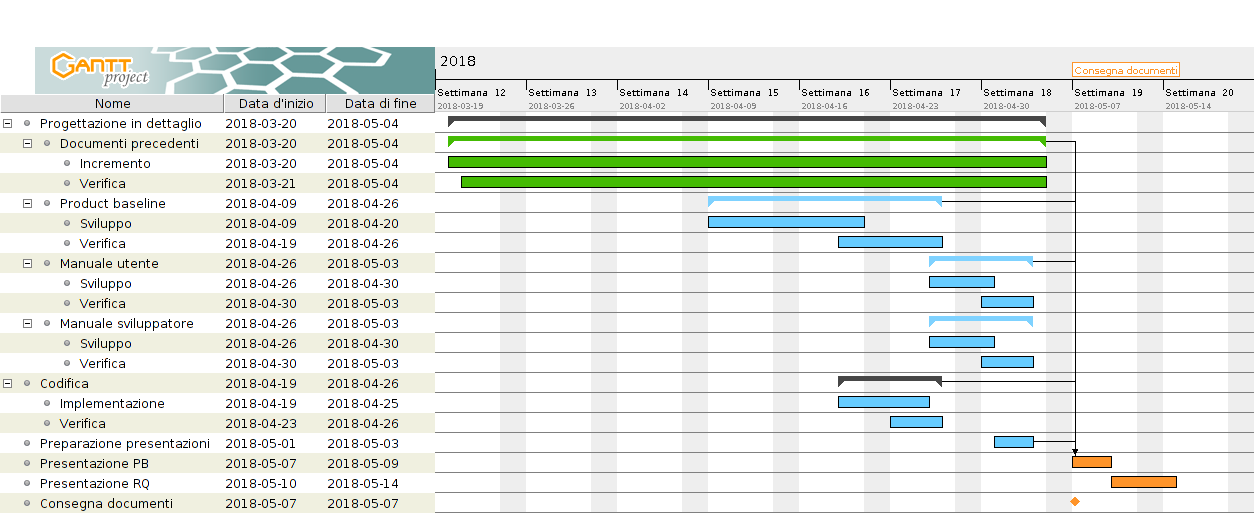
\includegraphics[width=1\linewidth, height=5cm]{./img/Gantt/ProgettazioneDettaglio.png}
                \caption[Gantt - Progettazione in dettaglio e codifica]{Diagramma di Gantt: Periodo di Progettazione in Dettaglio e Codifica}
            \end{figure}

	\newpage
	
	
	\subsection{Validazione e collaudo}
	\label{pianificazioneValidazione}
		L'ultimo periodo comincia successivamente alla consegna dei documenti
		richiesti in entrata alla \RQ{}, il 2018-05-15, e 
		si conclude il 2018-06-15 (\RA{}) con la consegna del prodotto completato 
		alla Proponente tramite supporto fisico (consegna materiale  2018-06-08). \\
		Le attività in questo periodo sono:

            \begin{itemize}
                \item \textbf{Incremento e verifica dei documenti precedenti:}
                    se necessario, verranno migliorati i documenti già scritti come
                    nel periodo precedente;
                \item \textbf{Incremento della progettazione e della codifica:}
                	per prepararsi alla revisione di accettazione il gruppo si occuperà di rendere
                	maturo il prodotto creato nel periodo precedente di progettazione in dettaglio
                	tramite incrementi nella progettazione e nella codifica. Raggiunto il grado massimo
                	di maturità dello stesso si potrà iniziare ad eseguire i test sul prodotto finale;
                \item \textbf{Esecuzione dei test:}
                    al fine di garantire la qualità di prodotto vengono effettuati
                    tutti i test descritti nel \PianoQualifica{}, che verrà aggiornato
                    di conseguenza;
                \item \textbf{Individuazione e correzione di bug};
                \item \textbf{Collaudo del prodotto finale}.
            \end{itemize}
	
            \begin{figure}[H]
                \centering
                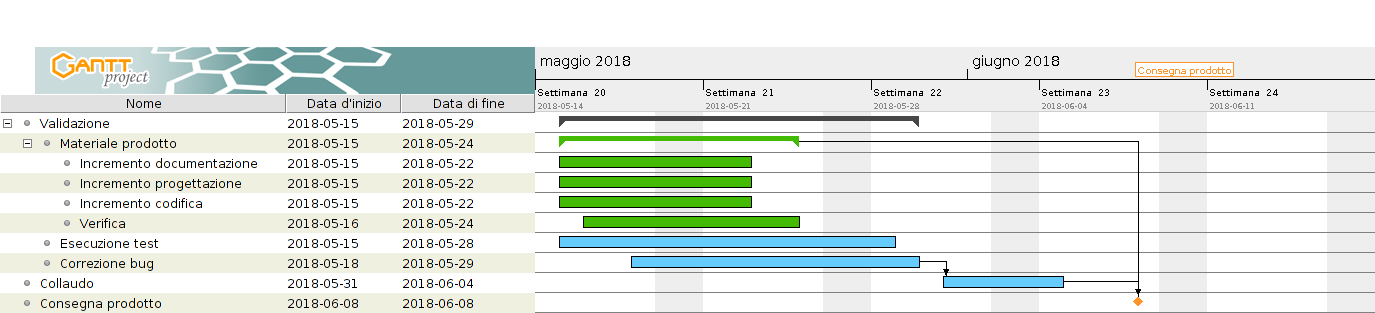
\includegraphics[width=1\linewidth, height=5cm]{./img/Gantt/Validazione.png}
                \caption[Gantt - Validazione e collaudo]{Diagramma di Gantt: Periodo di Validazione e Collaudo}
            \end{figure}

	\newpage